\chapter{L'outil de manipulation de texte rêvé}

Alors oui, pour ceux qui se demandent, je fais des rêves bizarres, mais bon chacun a ses petites tares cachées. Et rêver d'un outil qui améliore ma vie quotidienne en tant que codeur (ou écrivain, ou formateur, ou \ldots) n'est pas si étrange que ça.

Ce qui fait et fera encore le succès de \vim est sa capacité à \textbf{faciliter les manipulations de texte}. Certes il va vous proposer des fonctionnalités propres à chaque tâche que vous effectuerez \footnote{Souvent par l'intermédiaire de plugins.} comme la validation syntaxique de code, la correction orthographique, \ldots Mais à la fin, c'est toujours à écrire/corriger/manipuler/se déplacer dans du texte que vous passerez la majeure partie de votre temps. 

C'est là que l'approche de \vim est différente d'IDE comme Eclipse / Netbeans / PhpStorm et consœurs. Là où ces IDE vont mettre l'accent sur les particularités de votre langage de programmation tout en vous fournissant des capacités de manipulation de texte basiques, \vim adopte l'approche opposée : vous serez \textbf{très efficace} à manipuler/écrire du texte quelque soit le texte et vous pourrez enrichir \vim avec des fonctionnalités propres à votre langage de programmation via des plugins.

Nous allons donc voir dans ce chapitre comment utiliser \vim à bon escient (vous allez commencer à oublier votre souris) et quelle est la logique derrière tous ces enchaînements de commandes qui paraissent barbares au non initié. Vous devriez pouvoir, à la fin de ce chapitre, \textbf{vous passer de votre souris} pour éditer/manipuler le contenu d'un fichier\footnote{En tout cas, vous devriez vous forcer à le faire en apprenant \vim, ce n'est pas si dur que ça, et c'est ce qui fait la différence entre \vim et les autres : le tout clavier.}.

\section{Se déplacer par l'exemple : Essayer de copier / coller}\label{sec:se-deplacer}


Nous avons déjà vu dans la section «\nameref{sec:modeinsertion}» comment passer du mode insertion (pour saisir du texte) au mode normal (\emph{a priori} pour l'instant, vous ne savez pas trop à quoi sert ce mode). En appuyant sur \tti votre curseur passe en mode insertion (lorsque vous êtes en mode normal) et en appuyant sur \ttesc il repasse dans le mode normal. Bon bah on est bien Tintin. Et maintenant ? 

\subsection{Préambule}

Nous allons apprendre notre première manipulation de texte : le copier / coller. J'en vois certains d'entre vous se dire que ça ne sert à rien, car vous savez déjà le faire. Vous passez en mode insertion, vous prenez votre souris (ou vous vous déplacez avec les flèches directionnelles tout en appuyant sur \ttshift) pour sélectionner du texte et vous allez dans le \Verb|menu Édition| puis \Verb|Copier|. Et ensuite \Verb|menu Édition| puis \Verb|Coller|. Bah tiens, essayez pour voir.

Si vous avez suivi la section «\nameref{sec:modes}» traitant de la position idéale pour votre main, vous savez que vous avez fait une ou plusieurs choses que vous devriez vous interdire :


\begin{itemize}
    \item Vous avez utilisé votre souris
    \item Vous avez déplacé grandement votre main droite de sa position de repos, pour aller atteindre les flèches directionnelles qui sont très mal placées sur un clavier
\end{itemize}


Alors certes ce n'est pas grave en soit, mais c'est \textbf{inefficace} (se servir de la souris ou déplacer votre main droite vers les touches directionnelles est très lent) et \textbf{nuisible} pour vos petites mains. Si vous n'êtes pas prêt à vous forcer à ne pas le faire, je vous recommanderais presque d'\textbf{arrêter l'apprentissage de \vim} dès maintenant. \vim a été pensé pour ne pas utiliser la souris et pour ne pas bouger vos mains (ou presque). Ne pas se forcer à le faire, c'est ne pas utiliser \vim, et à un moment ou un autre, \textbf{vous le quitterez pour un éditeur} qui aura été pensé pour être utilisé à la souris. Alors, on continue ?

\subsection{Se passer de la souris}

Si vous lisez ces lignes c'est que vous avez répondu «oui», allons-y gaiement alors ! Nous allons tout d'abord commencer par nous passer de la souris. La prochaine étape sera de se passer des touches directionnelles, mais chaque chose en son temps.


\newthought{Pour réaliser un copier/coller} avec \vim tout se passe en mode «normal». Pour savoir dans quel mode vous vous trouvez, vous avez juste à regarder en bas à gauche de votre \vim. La figure \ref{fig:insert} vous montre \vim en mode «insertion» par exemple. Lorsque rien n'est marqué en bas à gauche, c'est que vous êtes en mode normal. Pour sortir d'un mode afin de retourner au mode normal, il suffit d'appuyer sur \ttesc\footnote{Si vous vous demandez pourquoi je vous dis d'arrêter d'utiliser la souris et/ou les touches directionnelles, mais que je ne dis rien sur le fait qu'il faille se torturer la main pour atteindre \ttesc, c'est que vous êtes sur la bonne voix. Je vous explique le comment du pourquoi dans «\nameref{sec:esc}».}.

\begin{figure}%
  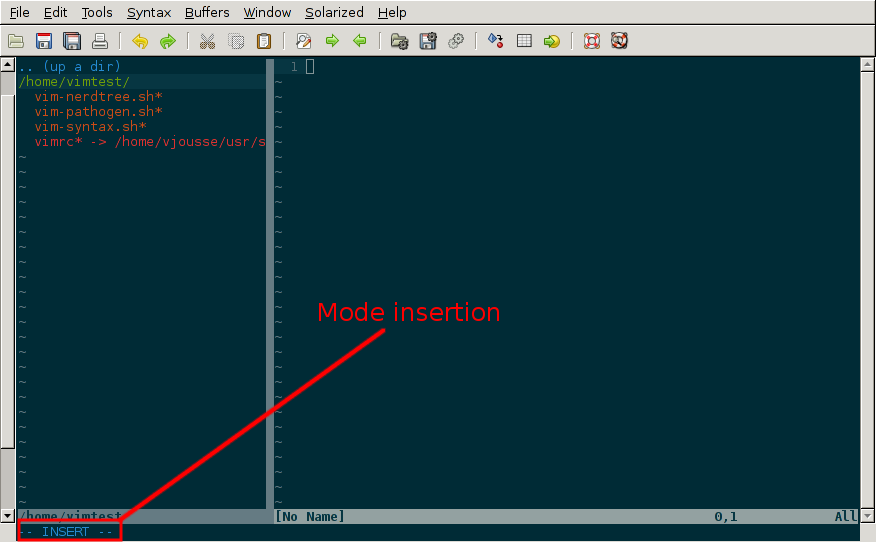
\includegraphics[width=\linewidth]{vim-insert.png}
  \caption{\vim en mode insertion.}
  \label{fig:insert}
\end{figure}

Admettons donc que vous êtes en mode «normal» et que vous avez un peu de texte de saisi dans votre \vim. Par exemple, cette chouette citation de Mark Twain : «Ils ne savaient que c'était impossible, alors ils l'ont fait.». Votre \vim devrait ressembler à celui de la figure \ref{fig:vim-twain}\footnote{Notez l'absence d'un quelconque mode d'affiché en bas à gauche.}.

\begin{figure}%
  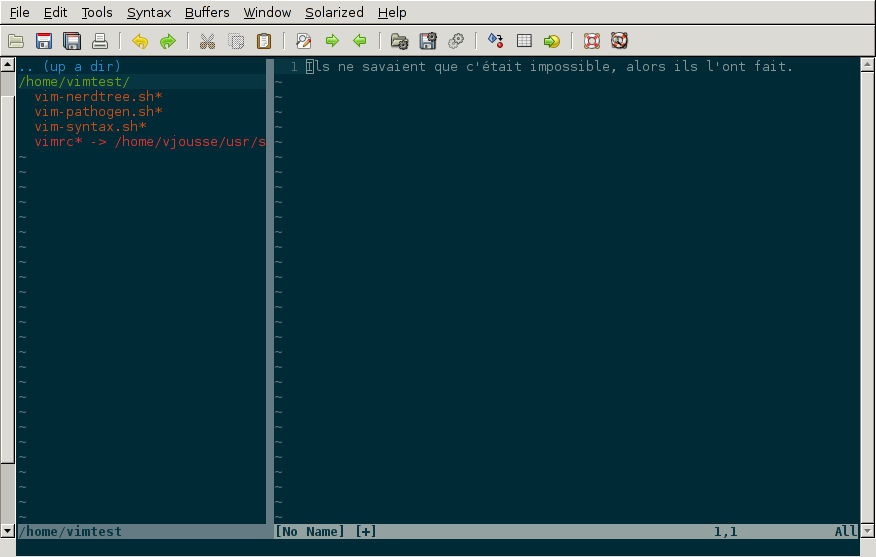
\includegraphics[width=\linewidth]{vim-twain.png}
  \caption{\vim prêt pour le copier/coller.}
  \label{fig:vim-twain}
\end{figure}

\section{Se passer des touches directionnelles}

\section{Se passer de la touche Échap}
\label{sec:esc}

\section{À vous de jouer}

\TODO exercices
